%label:"con:heegaardFloer"
%author:JeffHicks
%name:"construction of Heegaard Floer complex"
%type:"construction"

Let $(\Sigma_g, \underline{\alpha}, \underline{\beta})$ be a Heegaard diagram. Let $X=\Sym^g(\Sigma_g)$. Consider the submanifolds of $X$
\begin{align*}
    L_{\underline \alpha}:=\{[(z_1, \ldots, z_g)]\in X\st z_i\in \alpha_i\} && 
    L_{\underline \beta}:=\{[(z_1, \ldots, z_g)]\in X\st z_i\in \beta_i\}
\end{align*}
Since the $\alpha_i$ are disjoint from one another, this gives a smooth submanifold whose topology is $T^g$. Furthermore, since each of the $\alpha_i$ is a real subspace of $\Sigma_g$, the submanifold $L_\alpha$ is a real submanifold of $\Sigma_g$. A similar statement holds for $L_\beta$. \Cite{perutz2008handleslide} shows that $\Sym^g(\Sigma_g)$ can be equipped with a symplectic form which makes $L_{\underline \alpha},L_{\underline \beta}$ Lagrangian submanifolds. 

We wish to define the Heegaard-Floer cohomology as the Lagrangian intersection Floer cohomology of $L_{\underline \alpha},L_{\underline \beta}$. However, this is not an invariant of Heegaard diagrams --- note that isotopies of Heegaard diagrams give isotopies of Lagrangian submanifolds, while Lagrangian intersection Floer cohomology is only invariant under \emph{Hamiltonian isotopies} of Lagrangian submanifolds. We given an example exhibiting some of the problems with this preliminary approach.

%tag:0007
%label:exm:nonadmissibleHeegaardDiagram
%author:JeffHicks
%name:"Heegaard diagrams for $S^2\times S^1$"
%type:example


    We look at the example of $M=S^2\times S^1$. Observe that $S^2=D^2\cup_{S^1} D^2$, so we can write $M=D^2\times S^1 \cup_{\Sigma_1} D^2\times S^1$. 
    The Heegaard diagram $(\Sigma_1, \alpha, \beta)$ consists of a torus with two meridional cycles. 
    %label:"fig:nonadmissibleHeegaardDiagram"
%author:JeffHicks
%name:"non-admissible Heegaard Diagram"
%type:"figure"
%parent:"def:weaklyAdmissibleHeegaardDiagram"
%caption:"A non-admissible Heegaard diagram"


 

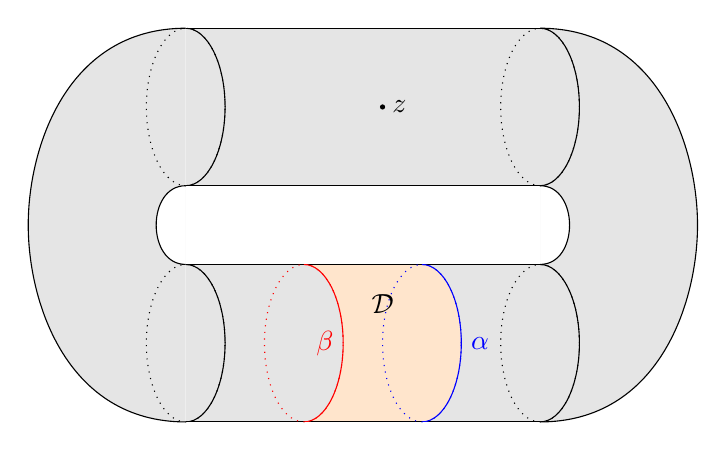
\begin{tikzpicture}



    \begin{scope}[]
    \begin{scope}[]
    
    \draw[fill=gray!20] (-2,-1.5) .. controls (-3.5,-1.5) and (-4,0) .. (-4,1) .. controls (-4,2) and (-3.5,3.5) .. (-2,3.5) (-2,1.5) .. controls (-2.5,1.5) and (-2.5,0.5) .. (-2,0.5);
    
    \end{scope}
    
    
    
    \begin{scope}[xscale=-1, shift={(-0.5,0)}]]
    
    \draw[fill=gray!20] (-2,-1.5) .. controls (-3.5,-1.5) and (-4,0) .. (-4,1) .. controls (-4,2) and (-3.5,3.5) .. (-2,3.5) (-2,1.5) .. controls (-2.5,1.5) and (-2.5,0.5) .. (-2,0.5);
    
    \end{scope}
    \fill[gray!20]  (-2,0.5) rectangle (2.5,-1.5);
    \fill[gray!20]  (-2,3.5) rectangle (2.5,1.5);

    \end{scope}
    
    \begin{scope}[]
    
    \fill[orange!20]  (1,-0.5) ellipse (0.5 and 1);
    \fill[orange!20]  (-0.5,0.5) rectangle (1,-1.5);
    \fill[gray!20]  (-0.5,-0.5) ellipse (0.5 and 1);
    \end{scope}
        \draw (-2,-1.5) -- (2.5,-1.5) (-2,0.5) -- (2.5,0.5) (-2,1.5) -- (2.5,1.5) (-2,3.5) -- (2.5,3.5);
    
    
    \begin{scope}[]
    
    \draw[dotted]  (-2,-0.5) ellipse (0.5 and 1);
    \clip  (-2,0.5) rectangle (-1,-1.5);
    \draw  (-2,-0.5) ellipse (0.5 and 1);
    \end{scope}
    
    
    
    \begin{scope}[red, shift={(1.5,0)}]
    
    \draw[dotted]  (-2,-0.5) ellipse (0.5 and 1);
    \clip  (-2,0.5) rectangle (-1,-1.5);
    \draw  (-2,-0.5) ellipse (0.5 and 1);
    \end{scope}
    
    
    \begin{scope}[blue, shift={(3,0)}]
    
    \draw[dotted]  (-2,-0.5) ellipse (0.5 and 1);
    \clip  (-2,0.5) rectangle (-0.5,-1.5);
    \draw  (-2,-0.5) ellipse (0.5 and 1);
    \end{scope}
    
    \begin{scope}[shift={(4.5,0)}]
    
    \draw[dotted]  (-2,-0.5) ellipse (0.5 and 1);
    \clip  (-2,0.5) rectangle (-1,-1.5);
    \draw  (-2,-0.5) ellipse (0.5 and 1);
    \end{scope}
    
    \begin{scope}[shift={(4.5,3)}]
    
    \draw[dotted]  (-2,-0.5) ellipse (0.5 and 1);
    \clip  (-2,0.5) rectangle (-1,-1.5);
    \draw  (-2,-0.5) ellipse (0.5 and 1);
    \end{scope}
    
    \begin{scope}[shift={(0,3)}]
    
    \draw[dotted]  (-2,-0.5) ellipse (0.5 and 1);
    \clip  (-2,0.5) rectangle (-1,-1.5);
    \draw  (-2,-0.5) ellipse (0.5 and 1);
    \end{scope}
    
    
    
    \node[left, red] at (0,-0.5) {$\beta$};
    \node[right, blue] at (1.5,-0.5) {$\alpha$};
    \node at (0.5,0) {$\mathcal D$};
    
    \node[circle, fill=black, scale=.2] at (0.5,2.5) {};
    \node[right] at (0.5,2.5) {$z$};
    
    \end{tikzpicture}
    If the diagram is chosen so that $\alpha, \beta$ are disjoint, then the Lagrangian intersection Floer cohomology $\HF(\alpha, \beta)$ vanishes.
    %label:"fig:admissibleHeegaardDiagram"
%author:JeffHicks
%name:"admissible HeegaardDiagram"
%type:"figure"
%parent:def:weaklyAdmissibleHeegaardDiagram
%caption:"An admissible Heegaard diagram"


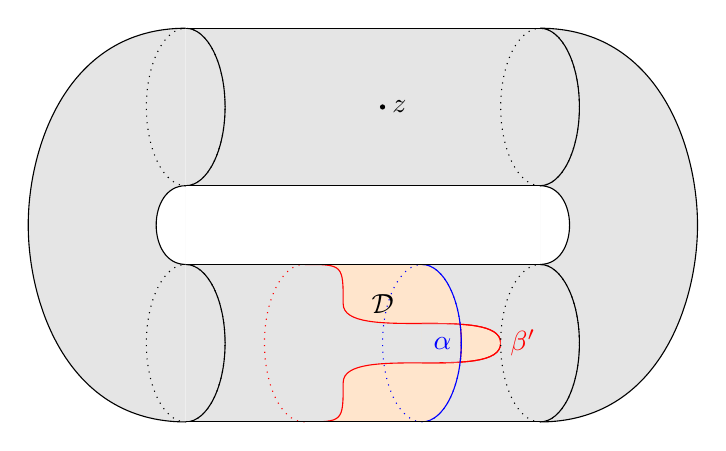
\begin{tikzpicture}

    \begin{scope}[]
    \begin{scope}[]
    
    \draw[fill=gray!20] (-2,-1.5) .. controls (-3.5,-1.5) and (-4,0) .. (-4,1) .. controls (-4,2) and (-3.5,3.5) .. (-2,3.5) (-2,1.5) .. controls (-2.5,1.5) and (-2.5,0.5) .. (-2,0.5);
    
    \end{scope}
    
    
    
    \begin{scope}[xscale=-1, shift={(-0.5,0)}]]
    
    \draw[fill=gray!20] (-2,-1.5) .. controls (-3.5,-1.5) and (-4,0) .. (-4,1) .. controls (-4,2) and (-3.5,3.5) .. (-2,3.5) (-2,1.5) .. controls (-2.5,1.5) and (-2.5,0.5) .. (-2,0.5);
    
    \end{scope}
    \fill[gray!20]  (-2,0.5) rectangle (2.5,-1.5);
    \fill[gray!20]  (-2,3.5) rectangle (2.5,1.5);
    
    \end{scope}
    
    \begin{scope}[]
    
    \fill[orange!20]  (1,-0.5) ellipse (0.5 and 1);
    \fill[orange!20]  (-0.5,0.5) rectangle (1,-1.5);
    \fill[gray!20]  (-0.5,-0.5) ellipse (0.5 and 1);
    \end{scope}
    
    
    \begin{scope}[]
    
    \draw[dotted]  (-2,-0.5) ellipse (0.5 and 1);
    \clip  (-2,0.5) rectangle (-1,-1.5);
    \draw  (-2,-0.5) ellipse (0.5 and 1);
    \end{scope}
    
    
    
    \begin{scope}[red, shift={(1.5,0)}]
    
    \draw[dotted]  (-2,-0.5) ellipse (0.5 and 1);
    \clip  (-2,0.5) rectangle (0.5,-1.5);
    \draw[fill=gray!20] (-2,0.5) .. controls (-1.5,0.5) and (-1.5,0.5) .. (-1.5,0) .. controls (-1.5,-0.5) and (0.5,0) .. (0.5,-0.5) .. controls (0.5,-1) and (-1.5,-0.5) .. (-1.5,-1) .. controls (-1.5,-1.5) and (-1.5,-1.5) .. (-2,-1.5);
    
    \clip  (-0.5,0) rectangle (0.5,-1);
    \draw[fill=orange!20] (-1.5,0) .. controls (-1.5,-0.5) and (0.5,0) .. (0.5,-0.5) .. controls (0.5,-1) and (-1.5,-0.5) .. (-1.5,-1);
    \clip (-1.5,0) .. controls (-1.5,-0.5) and (0.5,0) .. (0.5,-0.5) .. controls (0.5,-1) and (-1.5,-0.5) .. (-1.5,-1);
    
    \draw[fill=gray!20]  (-0.5,-0.5) ellipse (0.5 and 1);
    \draw (-1.5,0) .. controls (-1.5,-0.5) and (0.5,0) .. (0.5,-0.5) .. controls (0.5,-1) and (-1.5,-0.5) .. (-1.5,-1);
    
    \end{scope}
    
    
    \begin{scope}[blue, shift={(3,0)}]
    
    \draw[dotted]  (-2,-0.5) ellipse (0.5 and 1);
    \clip  (-2,0.5) rectangle (-0.5,-1.5);
    \draw  (-2,-0.5) ellipse (0.5 and 1);
    \end{scope}
    
    \begin{scope}[shift={(4.5,0)}]
    
    \draw[dotted]  (-2,-0.5) ellipse (0.5 and 1);
    \clip  (-2,0.5) rectangle (-1,-1.5);
    \draw  (-2,-0.5) ellipse (0.5 and 1);
    \end{scope}
    
    \begin{scope}[shift={(4.5,3)}]
    
    \draw[dotted]  (-2,-0.5) ellipse (0.5 and 1);
    \clip  (-2,0.5) rectangle (-1,-1.5);
    \draw  (-2,-0.5) ellipse (0.5 and 1);
    \end{scope}
    
    \begin{scope}[shift={(0,3)}]
    
    \draw[dotted]  (-2,-0.5) ellipse (0.5 and 1);
    \clip  (-2,0.5) rectangle (-1,-1.5);
    \draw  (-2,-0.5) ellipse (0.5 and 1);
    \end{scope}
    
    
    
    \node[right, red] at (2,-0.5) {$\beta'$};
    \node[left, blue] at (1.5,-0.5) {$\alpha$};
    \node at (0.5,0) {$\mathcal D$};
    
    \node[circle, fill=black, scale=.2] at (0.5,2.5) {};
    \node[right] at (0.5,2.5) {$z$};
    
    \draw (-2,-1.5) -- (2.5,-1.5) (-2,0.5) -- (2.5,0.5) (-2,1.5) -- (2.5,1.5) (-2,3.5) -- (2.5,3.5);
    
\end{tikzpicture}
    However, if the diagram is chosen so that $\alpha, \beta'$ intersect transversely, the Lagrangian intersection Floer cohomology (with $\ZZ/2\ZZ$ coefficients) is $\ZZ/2\ZZ\oplus \ZZ/2\ZZ$. Note that $\beta'$ can be chosen so that it is Hamiltonian isotopic to $\beta$.
    
    The discrepancy between these two answers comes from the non-convergence of the homotopy between the composition of continuation maps  $f\circ g:\CF(\alpha, \beta')\to \CF(\alpha, \beta) \to \CF(\alpha, \beta')$ and $\id: \CF(\alpha, \beta')$ over $\ZZ/2\ZZ$ coefficients. The presence of an annulus between $\alpha, \beta$ is the culprit for the non-convergence.

    If one instead chooses to use Novikov (instead of $\ZZ/2\ZZ$ coefficients) one can obtain a 

    To rule out this phenomenon, we only look at strips which avoid the marked point $z$, and will impose a criterion (admissible Heegaard diagrams) which will, in this setting, preclude the existence of annuli disjoint from the marked point $z$.  In general, the admissibility criterion will limit us to configurations of cycles for which the number of holomorphic strips contributing to the Floer differential is finite.




We desire the best of both worlds: invariance under Lagrangian isotopies, and convergence. In \cref{exm:nonadmissibleHeegaardDiagram} this can be achieved by only looking at strips which avoid the marked point $z$. When this marked point is chosen well, we will obtain a criterion (admissible Heegaard diagrams) which precludes the existence of annuli disjoint from the marked point $z$.  In general, the admissibility criterion will limit us to configurations of cycles for which the number of holomorphic strips contributing to the Floer differential is finite.

The marked point is introduced by slightly generalizing our definition of a Heegaard diagram. 
%label:"def:pointedHeegaardDiagram"
%author:JeffHicks
%name:"pointed Heegaard diagram"
%type:"definition"


    A \emph{pointed Heegaard diagram}  $(\Sigma_g, \underline \alpha, \underline \beta, z)$ is a Heegaard diagram $(\Sigma_g, \underline \alpha, \underline \beta)$ along with a choice of point $z$ disjoint from the cycles $\underline \alpha, \underline \beta$.

As a vector space, the Heegaard Floer cohomology of the pointed Heegaard diagram $(\Sigma,\underline{\alpha}, \underline{\beta},z)$ is
\[\HeF(\Sigma, \underline{\alpha}, \underline{\beta},z):=\bigoplus_{x\in L_{\underline \alpha}\cap L_{\underline{\beta}}} \ZZ/2\ZZ\langle x\rangle.\]
The differential is defined in a manner similar to the Lagrangian intersection Floer cohomology, but we will need to overcome the following difficulties.

\begin{itemize}
    \item Gromov-Compactness: Observe that this is defined over $\ZZ/2\ZZ$ coefficients. In general, when we look at the strips connecting two points $x, y$, we are only guaranteed compactness of the moduli space of pseudoholomorphic strips which have bounded energy. To get around this problem --- when strips from $x$ to $y$ have possibly unbounded energy --- we would employ Novikov coefficients in Lagrangian intersection Floer cohomology. Here, we do not use such a coefficient ring. 
    \item  If we treat $X$ as a symplectic manifold, the Lagrangian submanifolds $L_{\underline \alpha}, L_{\underline \beta}$ are not tautologically unobstructed (i.e. $\omega(\pi_2(X, L))\neq 0$). We therefore must rule out disk and sphere bubbling to show that the differential squares to zero.
\end{itemize}

The choice of base point defines a subset $Y_z\subset X$ given by  
\[ Y_z:=\{[(z, z_2, \ldots, z_g)] \st z_i\in \Sigma_g\} \subset X\]
which is disjoint from $L_{\underline \alpha}\cup L_{\underline \beta}$. Both issues above can be avoided by only looking at strips which are disjoint from $Y_z$.

For $x, y\in L_{\underline \alpha}\cap L_{\underline \beta}$ let $\mathcal M(x, y)$ denote the moduli space of holomorphic strips with boundary on $L_{\underline \alpha}\cup L_{\underline \beta}$, and ends limiting to $x$ and $y$. Let $\mathcal M(x, y)_{z=0}^0$ be the zero-dimensional component of $\mathcal M(x, y)$ consisting of strips which are disjoint from $Y_z$. The differential of Heegaard Floer cohomology is defined by the structure coefficients
\[\langle d_zx , y \rangle = \#\mathcal M(x, y)_{z=0}^0.\]
The following lemmas rule out the presence of disk and sphere bubbling.
%label:lem:heegaardNoSpheres
%author:JeffHicks
%name:"sphere bubbling in Heegaard differential"
%type:lemma


    Suppose that $g>2$. Then $\pi_2(\Sym^g(\Sigma_g))=\ZZ$. The generator of this group intersects $Y_z$.

%label:lem:heegaardNoDisks
%author:JeffHicks
%name:"disk bubbling in Heegaard differential"
%type:lemma



    Suppose that $u: D^2\to L_\alpha$ is a holomorphic disk. Then the image of $u$ intersects $Y_z$.

Provided that we can show that $(d_z)^2=0$, the Heegaard-Floer cohomology is defined to be the homology of the chain complex
\[\HHeF(M):= H^\bullet(\HeF(\Sigma, \underline \alpha, \underline \beta ,z), d_z).\]
As a result of these two lemmas, our restriction to counting disks which \emph{do not} pass through $Y_z$ gives us moduli spaces whose compactifications, if defined, would be free from disk and sphere bubbling. 

However, it remains to show that we have Gromov compactness.

